\chapter{Resultat}

\section{Produkt- och webbutveckling}
Från de första intervjuerna och utvärderingarna var resultatet att studenterna uppskattade den översikt och struktur som programmen ger. Var de däremot upplevde att de saknade var lösningsförslag och tips när man fastnar i lösningsgången. Från resultatet från benchmarkningen var att vara tydlig med feedback till användaren både visuell i form av gröna bockar och progression bars. Men även att hålla gränssnittet avskalat och inte dölja några element. 

Resultatet frontendmässigt går att se i bilderna nedan

\begin{center}
\begin{figure}[h]
    \centering
    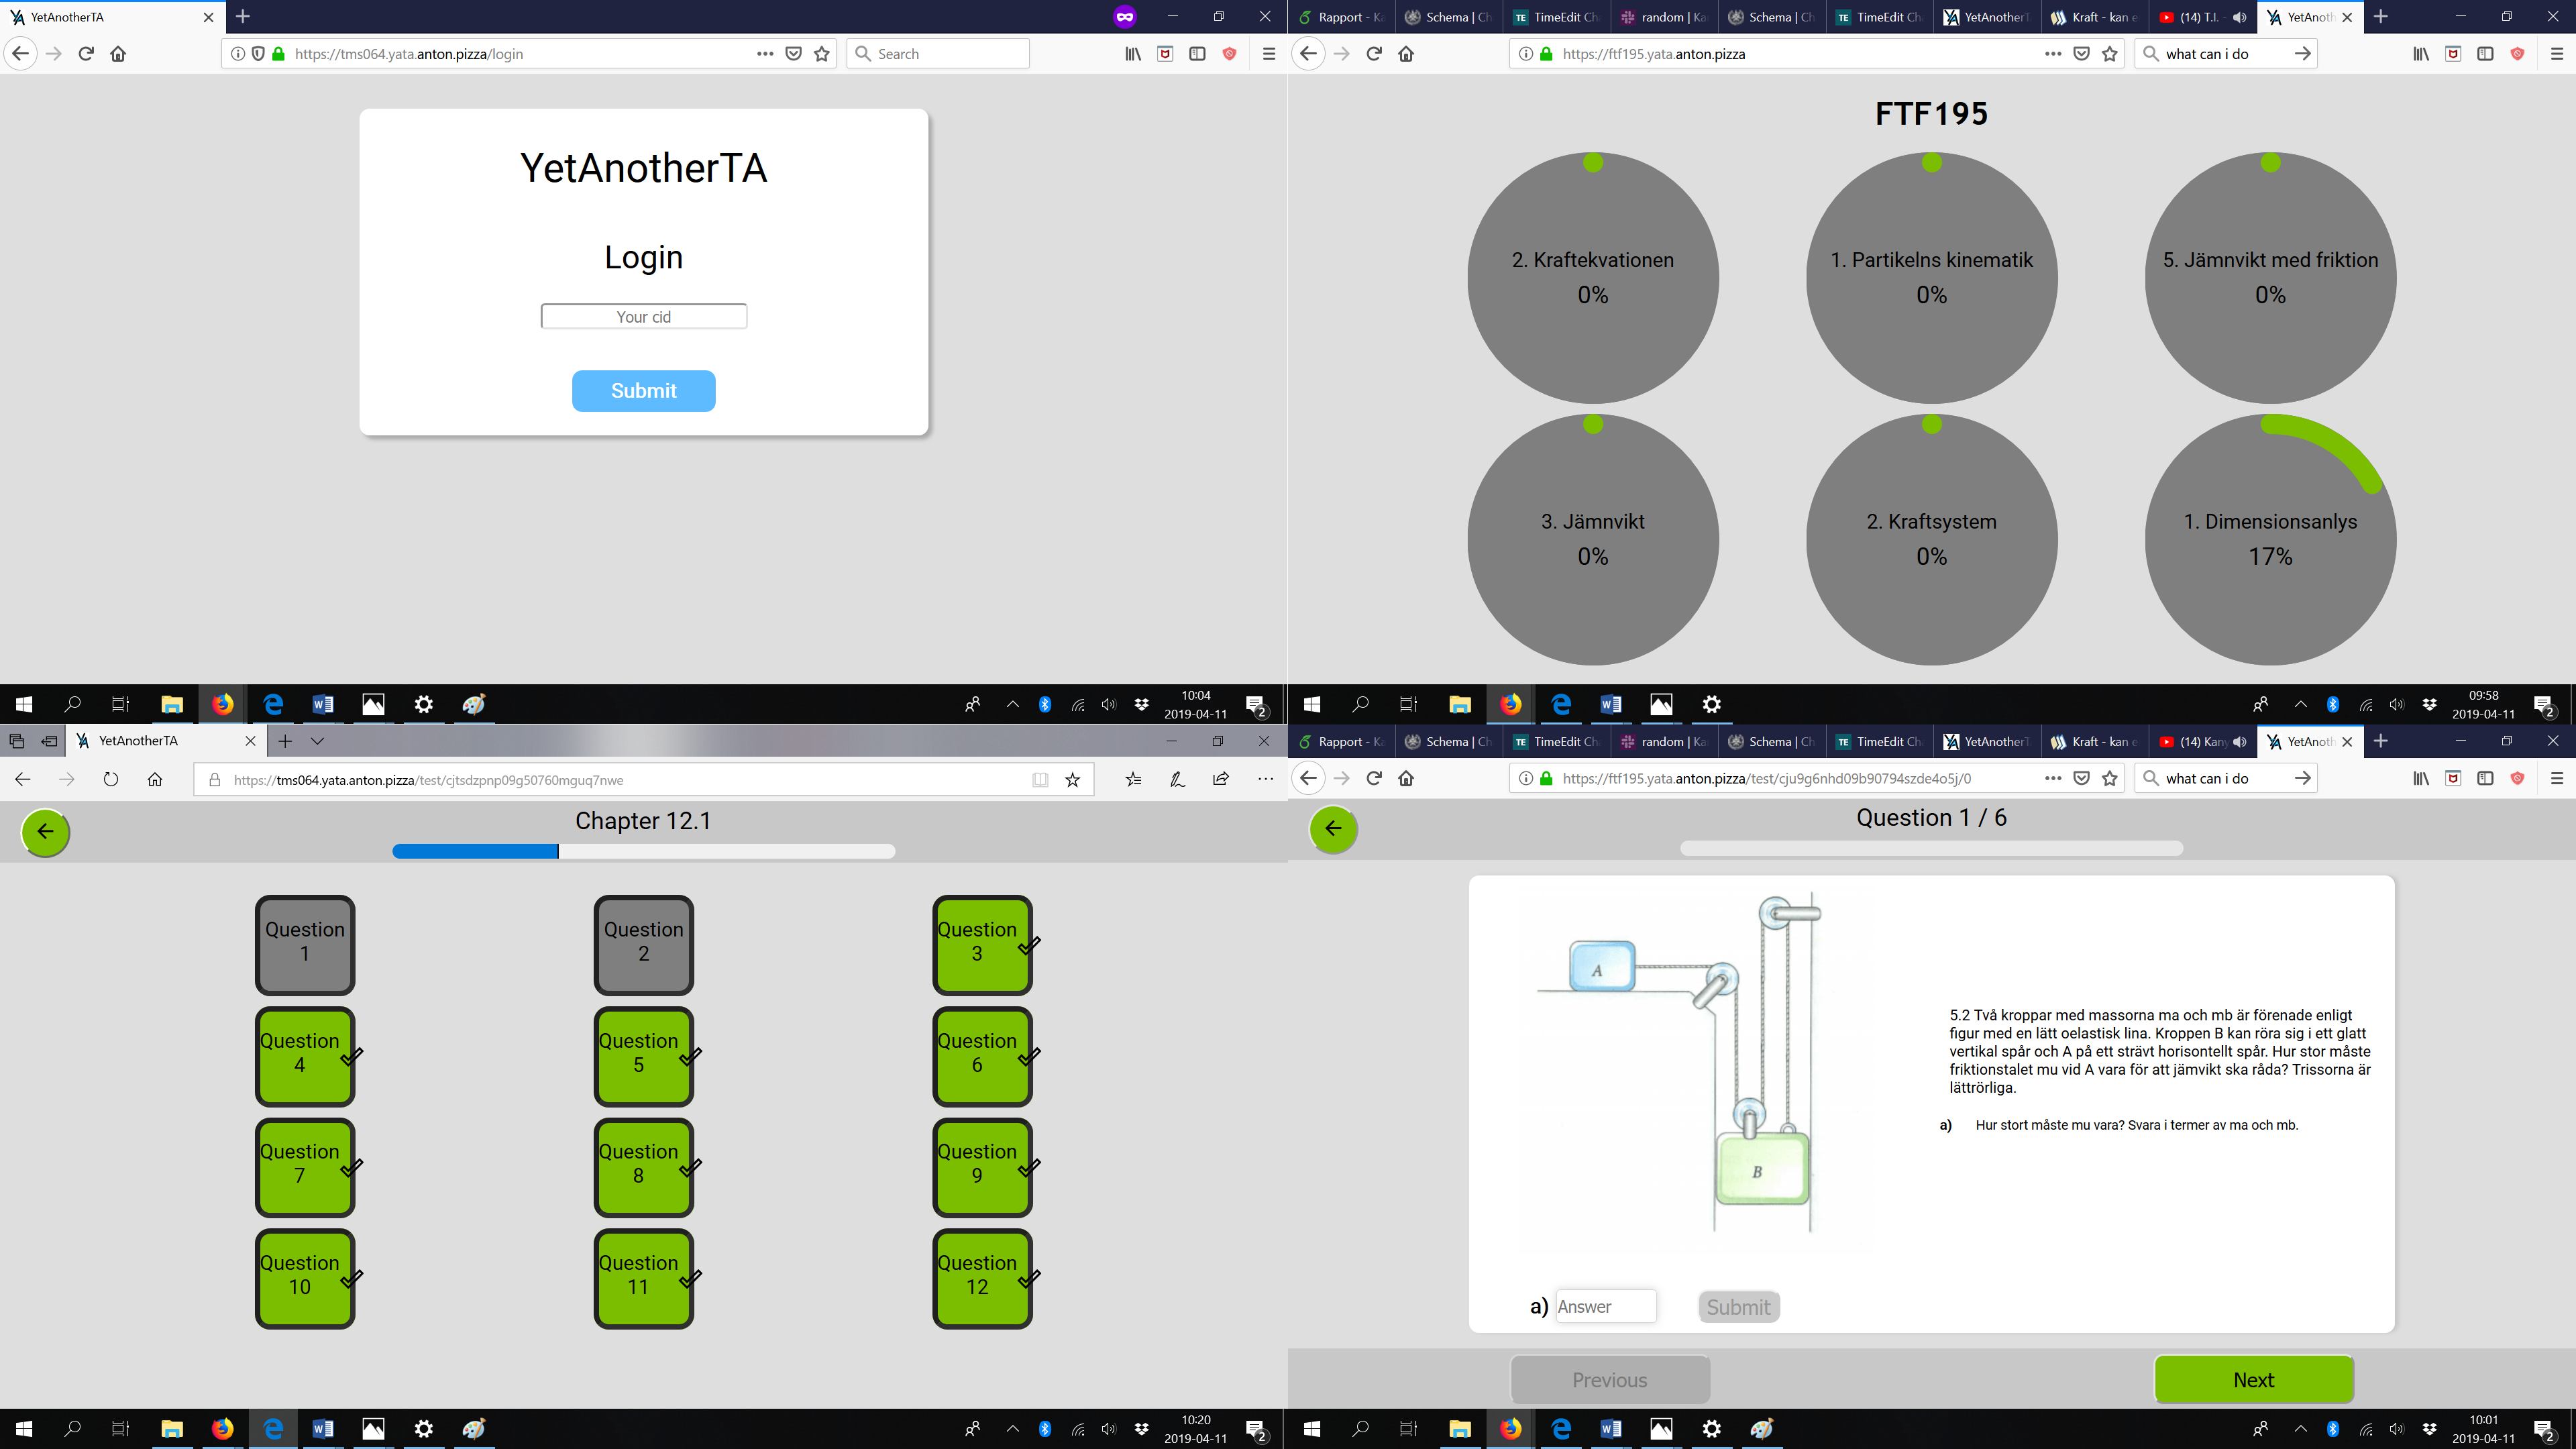
\includegraphics[width=1.0\textwidth]{images/resultpictures/4in1.png}
    \caption{Fyra skärmdumpar av hemsidan. I övre vänstra hörnet är loginskärmen, i övre högra hörnet översikt över kapitlen, i nedre vänstra översikt över uppgifterna i ett kapitel och i undre högra hörnet en vy över en uppgift. }
    \label{raket}
\end{figure}
\end{center}

%% Teknik, förklara hur klasser och requests representeras bildligt i figurerna ovan.

Användaren uppmanas till att mata in sitt CID, som sedan används i en nätverksförfrågan till databasen. Om användaren inte finns registrerad på kursen fås ett error-meddelande tillbaka. Annars omdirigeras användaren till översikts-vyn för tillgängliga frågesamlingar. I detta stadiet kan användaren välja bland de samlingar av uppgifter som presenteras, oftast som kapitel, eller tentamen. 

När användaren klickar på vald samling uppgifter, kommer ID:t för samlingen att användas med React Router, för att dirigera användaren till övesiktsvyn. Översiktsvyn visar samtliga frågor, och användaren kan även se vilka frågor som är besvarade. Klassen som vyn representerar, baseras mer eller mindre på samma sätt som föregående vy. En query skickas till Apollo-klienten, där frågorna för valt test återfås som en lista. Dessa målas då ut som fyrkanter, och är gröna ifall de har besvarats. Från föregående steg är alla frågor redan sparade i cache-minnet, eftersom listan av frågor innehåller all nödvändig information. Således innebär det att användaren kommer nå vyn för en specifik fråga direkt, utan att behöva vänta på en eventuell query. Klassen som hanterar frågevyn är uppdelad i tre delar: Header, Form och Footer. 

I Form presenteras frågan, med eventuell bild och svarsfält. Form är dynamiskt programmerad, för att alltid anpassa innehållet till skärmens storlek. I footer finns knappar för navigering mellan frågorna. Som tidigare nämnt, är alla frågor sparade i cache-minnet, vilket innebär att navigationen upplevs momentan. När användaren matar in ett svar i någon av fälten anropas funktionen sendAnswer. Metoden begär vid anrop en mutation från Apollo-klienten, som först lägger till svaret i databasen, för att sedan returnera om svaret var rätt eller fel. Responsen kommer i klassen sedan motsvaras av en grön bock eller ett rött kryss, som användaren ser. 

Eftersom studenterna uppskattade översikt och struktur är detta något som har prioriterats i designen. Efter att man loggat in ska man i kapitelvyn snabbt kunna få en överskådlig bild av hur man ligger till i kursen. Detta genom att man ser de olika kapitlen samt hur långt man har kommit genom en procentsats samt en progression bar. Går man in på ett kapitel kommer man till en översikt över de olika uppgifterna i kapitlet. Man se där hur många uppgifter kapitlet innehåller samt vilka som är lösta respektive olösta. Överst i denna skärm ser man en progression bar över hur långt man har kommit i kapitlet. I översiktsvyn har man en bild till vänster samt text till höger. Överst ser man samma progression bar som visar hur långt man har kommit i kapitlet. 

Från utvärderingen från första kursen i läsperiod 3 mottogs en del feedback för att förbättra anvädningen. Till exempel att ett svar ska stå kvar i rutan då man kommer tillbaka till uppgiften senare, eller tydligare feedback om man gjort fel svar två gånger i rad. För fulla listan av förbättringspunkter, se appendix. 

Resultatet från brukarstudien av Plattformen Piazza går att se i diagram x. Slutsatsen var att Piazza inte användes så mycket som man kunde tänka sig. Vi identifierade flera anledningar till detta, till exempel att många är rädda för att ställa en fråga i forumet, men också på grund av att svarstiden är långsam. Vi identifierade en form av hierarki efter hur man söker efter hjälp när man kört fast. Många börjar med att googla på problemet, hittar man ingen hjälp där, kanske man frågar i en Messengerchatt med sina närmsta kompisar. Hittar man det inte där kanske man frågar en annan kursare och sista utvägen är att fråga på Piazza. En tolkning av detta är att studenterna värdesätter svarstiden högre än kvalitén på svaren

Utifrån den insamlade informationen föreslogs ett antal koncept som skulle kunna uppfylla de behov vi såg, se appendix för lista. Det koncept vi slutligen gick för är en typ av tipsfunktion. Detta med tanke på dels att studenterna efterfrågade tips i första utvärderingen av OpenTA, men också att det kanske är ett mycket snabbt sätt att få hjälp om man har kört fast. Tanken är att den som löst en uppgift får möjligheten att skriva in ett tips för hur man löste den. Om någon då har kört fast på samma uppgift kan den personen då efterfråga ett tips.

%%Tekniskt stycke, hur funkar tipsfunktion rent kodmässigt med klasser och requests
Tips-funktionen förändrar inget av den tidigare beskrivna implementationen, utan motsvarar endast tillagd funktionalitet. När användaren trycker på tips-knappen renderas modal-panelen där tipsen syns, och en query skickas till Apollo-klienten, där svaret innehåller det högst röstade tipset. Användaren kan sedan navigera mellan tipsen, och vid en eventuell rörelse kommer en ny query skickas till Apollo-klienten på samma sätt. Anledningen till att alla tips inte sparas i cache-minnet är av två skäl. 

Först och främst hade det inneburit att en användare med enklare erfarenheter av webbutveckling kan komma åt samtliga tips i nätverksloggen, vilket i sin tur innebär att deep learning-algoritmen inte med säkerhet kan veta om användaren tagit hjälp av tips. För det andra hade det även försvårat processen att manuellt avgöra hur många tips en användare tagit hjälp av. För enkelhetens skull kan istället anropet till Apollo-klienten för varje tips användas som referens till algoritmen.

En användare kan även rösta på existerande tips, för att förbättra relevansen hos tipsen. De två "tummarna" motsvarar då antingen +1 eller -1. När en användare röstar anropas en liknande mutation som vid ovan nämnt bevarande av en fråga. I mutationen skickas antingen +1 eller -1, och responsen innehåller tipset användaren röstat på. Detta för att uppdatera cache-minnet (med enbart den frågan), eftersom då användaren kan se förändringar.

När en användare besvarat samtliga delfrågor för en uppgift, visas en en modal där användaren uppmanas dela sitt mest betydelsefulla tips för frågan. Anledningen bakom att uppmana användaren på ett så "avbrytande" vis, är för att fånga så många svar som möjligt. Ett problem hade annars varit att användaren inte ser något värde i att lämna tips.

När användaren väljer att lämna ett tips anropas en mutation till Apollo-klienten, som tar in svaret, och returnerar resultatet i form av en boolsk variabel.



\section{Dataanalys}

\section{Förutsägelse av godkänt eller underkänt (U, G)}

\section{Förutsägelse av betyg (U, 3, 4, 5)}

\section{Felanalys av förutsägelserna}

\section{Applicering av arkitekturer baserade på LSTM-lager}

\section{Förutsägelse av skrivningspoäng och osäkerhetsnätverk}
I följande avsnitt presenteras förutsägelserna av skrivningspoäng för skrivningspoängsnätverken och framtagna osäkerhetsnätverk vilka presenterades i avsnitt \ref{sec:exam_score}. Först diskuteras resultaten för datamängden ifrån kursen FFM234 och därefter resultaten för datamängden ifrån kursen FFM521.

\begin{figure}[H]
    \centering
    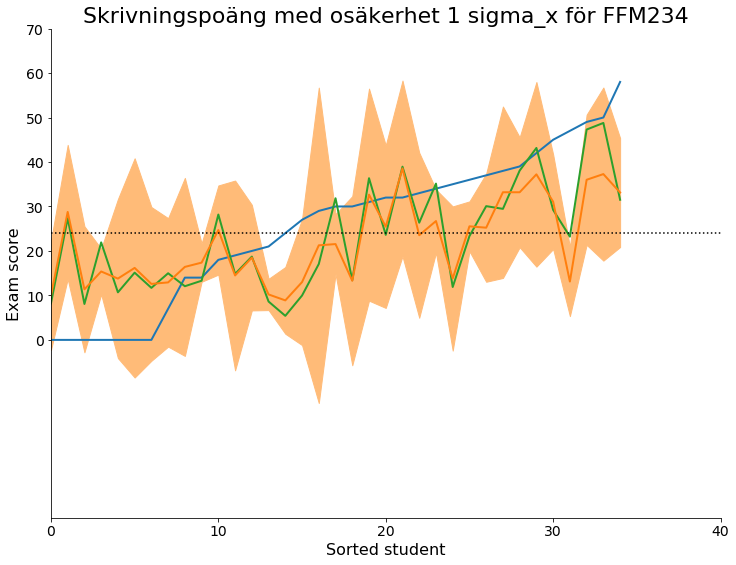
\includegraphics[width=0.8\textwidth]{images/resultpictures/Osakerhetsgraf-FFM234-1.png}
    \caption{Verkliga skrivningspoäng (blå) och förutsagda skrivningspoäng enligt skrivningspoängsnätverken (grön) och osäkerhetsnätverk (orange) för kursen FFM234. Det orange skuggade området motsvarar en standardavvikelse för aleatoriska osäkerheten $\sigma_x$. Notera att den linjerade svarta linjen motsvarar gränsen för godkänt i kursen.}
    \label{fig:exam_score_results_ffm234}
\end{figure}
Förutsägelserna av skrivningspoäng i kursen FFM234 visas i figur \ref{fig:exam_score_results_ffm234}. Skrivningspoängsnätverket presterar förutsägelser med ett medelabsolutfel (MAE) $E = \sum_{i=1}^N \left|y_i - \hat{y}_i\right| = 10.2\,\rm poäng$. Osäkerhetsnätverket presterar förutsägelser med ett medelabsolutfel $E = 11.3\,\rm poäng$. Osäkerhetsnätverket uppskattar i medel den aleatoriska osäkerheten till $\sigma_x = 14.7\,\rm poäng$.

Vidare presenteras förutsägelserna av skrivningspoäng i kursen FFM521 i figur \ref{fig:exam_score_results_ffm521}.
\begin{figure}[H]
    \centering
    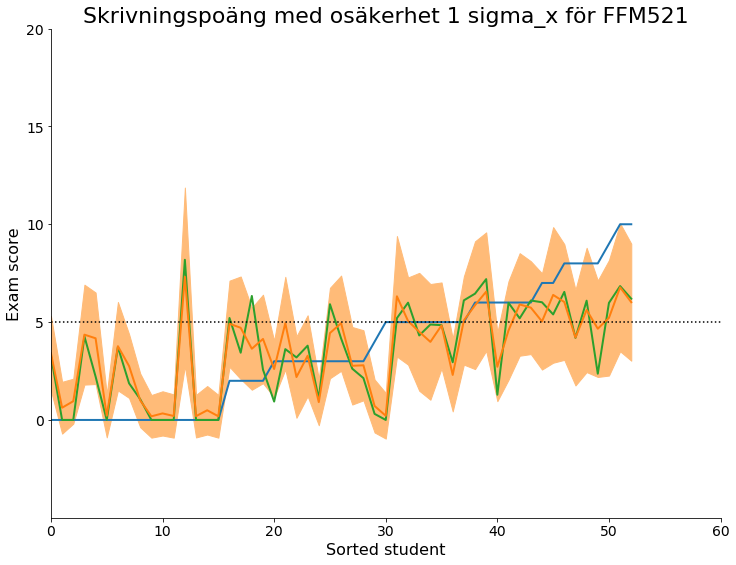
\includegraphics[width=0.8\textwidth]{images/resultpictures/Osakerhetsgraf-FFM521-1.png}
    \caption{Verkliga skrivningspoäng (blå) och förutsagda skrivningspoäng enligt skrivningspoängsnätverken (grön) och osäkerhetsnätverk (orange). Det orange skuggade området motsvarar en standardavvikelse för aleatoriska osäkerheten $\sigma_x$. Observera att den linjerade svarta linjen motsvarar gränsen för godkänt i kursen.}
    \label{fig:exam_score_results_ffm521}
\end{figure}
Notera att maximala skrivningpoängen för kursen FFM521 är 15 poäng medan maximala skrivningspoängen för kursen FFM234 är 60 poäng. Därav varierar storleken av medelabsolutfel och aleatorisk osäkerhet mellan kurserna. Skrivningspoängsnätverket ger förutsägelser med medelabsolutfel $E = 1.73\,\rm poäng$ och osäkerhetsnätverket presterar förutsägelser med det jämförbara felet $E = 1.77\,\rm poäng$. Osäkerhetsnätverket uppskattar medelvärdet av den aleatoriska osäkerheten till $\sigma_x = 2.18\,\rm poäng$. 

